\documentclass[tikz,border=4pt]{standalone}
\usepackage{amsmath}
\usepackage{amssymb}
\usetikzlibrary{arrows.meta,backgrounds,calc,fit}

\definecolor{tsorange}{RGB}{224,148,82}
\definecolor{wiregray}{RGB}{76,80,82}
\definecolor{sepgray}{RGB}{150,150,150}

\begin{document}
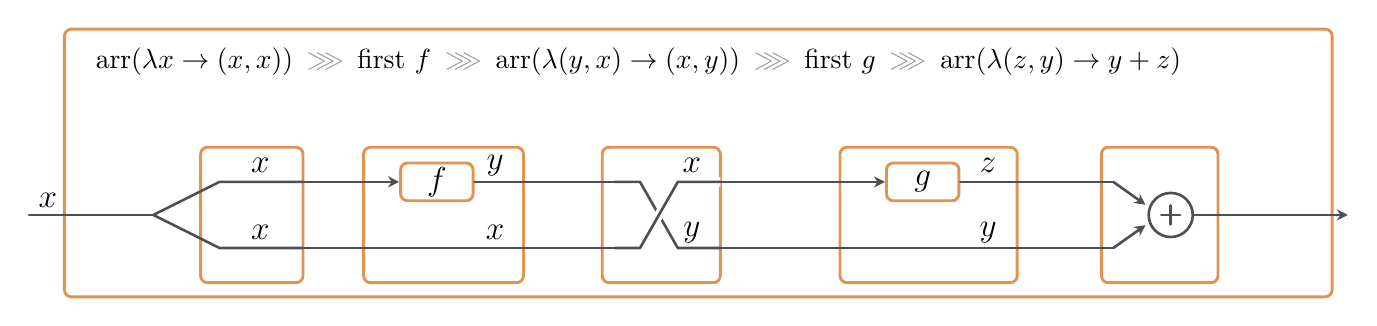
\begin{tikzpicture}[
  x=1cm,
  y=1cm,
  wire/.style={
    draw=wiregray,
    line width=0.95pt,
    line cap=round,
    line join=round
  },
  wire arrow/.style={
    wire,
    -{Stealth[length=4pt,width=4pt]}
  },
  op box/.style={
    draw=tsorange,
    rounded corners=2.5pt,
    line width=1.05pt,
    inner sep=0pt
  },
  fun box/.style={
    op box,
    minimum width=0.92cm,
    minimum height=0.48cm,
    inner sep=1pt,
    font=\large,
    fill=white
  },
  wire label/.style={
    font=\large,
    inner sep=0.7pt,
    fill=white
  },
  formula op/.style={
    anchor=base west,
    font=\normalsize,
    inner sep=0pt
  },
  formula sep/.style={
    formula op,
    text=sepgray
  },
  above wire/.style={wire label, anchor=south, yshift=1.7pt},
  below wire/.style={wire label, anchor=north, yshift=-1.7pt},
  pics/duplicate/.style={
    code={
      \draw[wire] (-1.58,0) -- (0,0);
      \draw[wire] (0,0) -- (0.84,\wireupper) -- (1.90,\wireupper);
      \draw[wire] (0,0) -- (0.84,\wirelower) -- (1.90,\wirelower);
      \node[wire label] at (-1.34,0.18) {$x$};
      \node[wire label] at (1.36,0.63) {$x$};
      \node[wire label] at (1.36,-0.22) {$x$};
    }
  },
  pics/swap/.style={
    code={
      \draw[wire] (0,\wireupper) -- (0.32,\wireupper) --
        (0.80,\wirelower) -- (1.34,\wirelower);
      \draw[wire, preaction={draw=white, line width=3.4pt}]
        (0,\wirelower) -- (0.32,\wirelower) --
        (0.80,\wireupper) -- (1.34,\wireupper);
    }
  },
  pics/sum/.style={
    code={
      \draw[wire arrow] (-0.73,\wireupper) -- (-0.32,0.13);
      \draw[wire arrow] (-0.73,\wirelower) -- (-0.32,-0.13);
      \draw[wire] (0,0) circle[radius=0.28];
      \draw[wire] (-0.12,0) -- (0.12,0);
      \draw[wire] (0,-0.12) -- (0,0.12);
    }
  }
]

\def\wireupper{0.42}
\def\wirelower{-0.42}
\def\boxtop{0.86}
\def\boxbottom{-0.86}

% Named box corners.  The boxes are drawn later using TikZ's fit library.
\coordinate (outer-sw) at (-0.55,-1.04);
\coordinate (outer-ne) at (15.55,2.36);
\foreach \boxname/\xmin/\xmax in {
  dup/1.18/2.48,
  firstf/3.25/5.28,
  swap/6.28/7.78,
  firstg/9.30/11.55,
  merge/12.62/14.10
}{
  \coordinate (\boxname-sw) at (\xmin,\boxbottom);
  \coordinate (\boxname-ne) at (\xmax,\boxtop);
}

\coordinate (formula-start) at (-0.16,1.86);
\node[formula op] (formula-a) at (formula-start)
  {$\operatorname{arr}(\lambda x \to (x,x))$};
\node[formula sep] (formula-s1) at ($(formula-a.base east)+(0.16,0)$)
  {$\ggg$};
\node[formula op] (formula-b) at ($(formula-s1.base east)+(0.16,0)$)
  {$\operatorname{first}\, f$};
\node[formula sep] (formula-s2) at ($(formula-b.base east)+(0.16,0)$)
  {$\ggg$};
\node[formula op] (formula-c) at ($(formula-s2.base east)+(0.16,0)$)
  {$\operatorname{arr}(\lambda(y,x)\to(x,y))$};
\node[formula sep] (formula-s3) at ($(formula-c.base east)+(0.16,0)$)
  {$\ggg$};
\node[formula op] (formula-d) at ($(formula-s3.base east)+(0.16,0)$)
  {$\operatorname{first}\, g$};
\node[formula sep] (formula-s4) at ($(formula-d.base east)+(0.16,0)$)
  {$\ggg$};
\node[formula op] (formula-e) at ($(formula-s4.base east)+(0.16,0)$)
  {$\operatorname{arr}(\lambda(z,y)\to y+z)$};

\begin{scope}[on background layer]
  \node[op box, fit=(outer-sw)(outer-ne)] {};
  \foreach \boxname in {dup,firstf,swap,firstg,merge}{
    \node[op box, fit=(\boxname-sw)(\boxname-ne)] {};
  }
\end{scope}

\node[fun box] (f) at (4.18,\wireupper) {$f$};
\node[fun box] (g) at (10.35,\wireupper) {$g$};

% arr (\lambda x -> (x,x)): duplicate the input.
\pic at (0.58,0) {duplicate};

% first f: apply f to the upper component, keep the lower component.
\draw[wire arrow] (2.48,\wireupper) -- (f.west);
\draw[wire] (f.east) -- (5.28,\wireupper);
\draw[wire] (2.48,\wirelower) -- (5.28,\wirelower);
\node[wire label] at (4.92,0.63) {$y$};
\node[wire label] at (4.92,-0.22) {$x$};

% arr (\lambda(y,x) -> (x,y)): swap the two components.
\draw[wire] (5.28,\wireupper) -- (6.44,\wireupper);
\draw[wire] (5.28,\wirelower) -- (6.44,\wirelower);
\pic at (6.44,0) {swap};
\draw[wire] (7.78,\wireupper) -- (9.30,\wireupper);
\draw[wire] (7.78,\wirelower) -- (9.30,\wirelower);
\node[wire label] at (7.42,0.63) {$x$};
\node[wire label] at (7.42,-0.22) {$y$};

% first g: apply g to the upper component, keep the lower component.
\draw[wire arrow] (9.30,\wireupper) -- (g.west);
\draw[wire] (g.east) -- (11.55,\wireupper);
\draw[wire] (9.30,\wirelower) -- (11.55,\wirelower);
\node[wire label] at (11.18,0.63) {$z$};
\node[wire label] at (11.18,-0.22) {$y$};

% arr (\lambda(z,y) -> y+z): merge the two components.
\draw[wire] (11.55,\wireupper) -- (12.77,\wireupper);
\draw[wire] (11.55,\wirelower) -- (12.77,\wirelower);
\pic at (13.50,0) {sum};
\draw[wire arrow] (13.78,0) -- (15.75,0);

\end{tikzpicture}
\end{document}
